\documentclass{standalone}

\usepackage{tikz}
\usepackage{tkz-euclide}

\usepackage{times}

\begin{document}
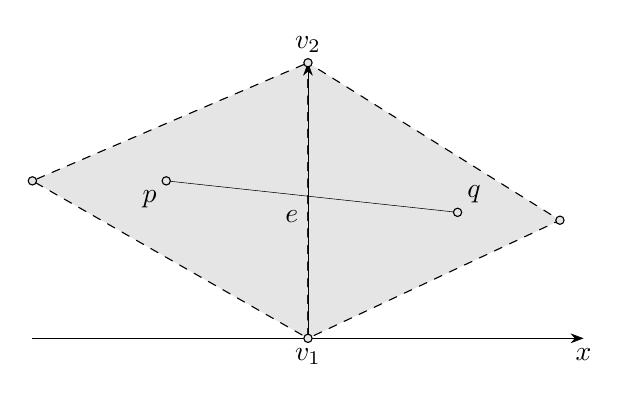
\begin{tikzpicture}[%
  line/.style = {thin, dotted},
  >={Stealth[scale=1.2]},
]

  \tkzDefPoint(0.0, 0.0){A}
  \tkzDefPoint(0.0, -3.5){B}
  \tkzDefPoint(-3.5, -1.5){C}
  \tkzDefPoint(3.2, -2.0){D}

  \tkzDefPoint(-3.5,-3.5){L}
  \tkzDefPoint(3.5,-3.5){R}
  \tkzDrawSegment[->](L,R)
  \tkzLabelPoint[below](R){$x$}

  \tkzDefPoint(-1.8, -1.5){P}
  \tkzDefPoint(1.9, -1.9){Q}

  \tkzDefPoint(1.6, 0.0){X}

  % \tkzInterLL(A,D)(B,C)
  % \tkzGetPoint{H}

  % \tkzInterLL(X,Q)(C,B)
  % \tkzGetPoint{HH}

  \tkzDrawPolygon[thin,dashed,fill=gray!20](A,B,C)
  \tkzDrawPolygon[thin,dashed,fill=gray!20](A,B,D)
  % \tkzDrawSegment[thin,dotted](A,H)
  % \tkzDrawSegments[thin](H,D D,B)

  \tkzDrawSegment(P,Q)
  % \tkzDrawSegment[dotted](X,HH)
  % \tkzDrawSegment(HH,Q)

  \tkzDrawSegment[->](B,A)
  \tkzLabelSegment[below left](B,A){$e$}

  \tkzLabelPoint[below](B){$v_1$}
  \tkzLabelPoint[above](A){$v_2$}
  \tkzLabelPoint[below left](P){$p$}
  \tkzLabelPoint[above right](Q){$q$}

  \tkzDrawPoints[size=3.0](A,B,C,D,P,Q)

\end{tikzpicture}
\end{document}
